\documentclass[11pt,letterpaper]{article}
\usepackage[margin=1.0in]{geometry}
\usepackage[utf8]{inputenc}
\usepackage{cite}
\usepackage{amsmath}
\usepackage{amsfonts}
\usepackage{amssymb}
\usepackage{makeidx}
\usepackage{graphicx}
\usepackage{hyperref}
\setlength\parindent{0pt}

\author{STUDENT NAME}
\title{Lab8: Temperature measurement using LabVIEW®}

\begin{document}

\maketitle

\section{Objectives}

This lab is designed to give students experience in LabVIEW®, with an application of temperature measurement.\\

The objectives of this lab are:\\

\begin{enumerate}
\item To understand the development environment of LabVIEW® using a front panel and a block diagram.
\item Gain experience in building an accurate temperature sensing circuit containing a commercially available thermistor (semiconductor temperature sensor) using its data sheet.
\item Understand the importance of standards and calibration, here using the triple point of water.
\end{enumerate}

\section{Introduction}
Temperature measurements are very common in industry. The standard for temperature measurement is documented in the \href{http://en.wikipedia.org/wiki/International_Temperature_Scale_of_1990}{International Temperature Scale of 1990 (ITS-90)} . The most common temperature sensor is the thermocouple, due to its wide range, and relatively low costs. However, thermocouple systems require special attention to details such as metal-metal interfacing, and reference junctions.\\

A simpler method is to use a low-cost semiconductor transducer such as the LM 135/235/335 Precision Temperature Sensor. These devices give a voltage output that can be measured using a Analog/Digital converter. The voltage output of the sensor is directly related to the absolute temperature in Kelvin, meaning at 0 deg C, the output is 2.732 V which in Kelvin is 273.15K. In addition, the output changes at a rate of 0.1V per deg C (or K, Kelvin and Celsius have the same slope), which means the nominal value at 25C is 2.982 Volt. To use the sensor, we can now simply multiply the measured voltage by 100, to obtain the temperature in Kelvin. To convert to Celsius, we subtract 273.15, and to convert from Celsius to Fahrenheit we use the conversion formula:\\

\begin{equation}
F = \dfrac{9}{5}C + 32
\end{equation}

The pin layout of the LM335 chip as well as a basic temperature sensor configuration is shown in Figure \ref{fig:Lab8_TemperatureMeasurementUsingLabVIEW_LM335PinLayout_TemperatureMeasurement}. Full specs can be found \href{http://abe-research.illinois.edu/Faculty/grift/ABE425_2015/Specs/LM335.pdf}{here}.

\begin{figure}
\centering
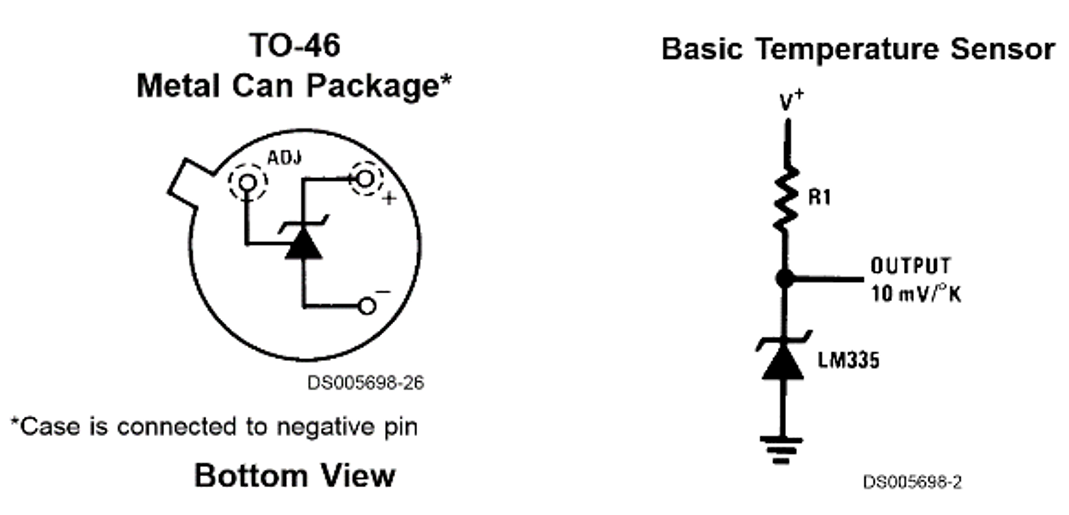
\includegraphics[width=1\linewidth]{Lab8_TemperatureMeasurementUsingLabVIEW_LM335PinLayout_TemperatureMeasurement}
\caption{Left: Pin layout of the LM335 chip. Right: Basic temperature sensor configuration.}
\label{fig:Lab8_TemperatureMeasurementUsingLabVIEW_LM335PinLayout_TemperatureMeasurement}
\end{figure}

In this lab we are using National Instruments’ LabVIEW®, a common data acquisition and analysis tool used in industry and academia. LabVIEW® has a graphical programming environment that can be learned quickly. Every LabVIEW® ‘Virtual Instrument’ consists of a Front Panel in which you can define the user interface using pictorials, and a Block Diagram, which shows the connectivity among the system components. One of the drawbacks of a graphical programming language is that producing an impressive looking user interface is easy, but to make the program work in the background can be quite challenging. 

\section{Equipment}

\begin{enumerate}
\item Computer with LabVIEW® software.
\item National Instruments USB 6008 DAQ board.
\item LM135/335 Precision Temperature Sensor.
\item Digital Multimeter.
\item Breadboard.
\item Cup with water and melting ice cubes.
\end{enumerate}

\section{Procedures}	 
\begin{enumerate}
\item Build the temperature sensing circuit. You will receive an LM135/335 thermistor and a 5.6k resistor for $R_1$.  The sensor requires a +5.0 V power supply, which you have to get from the Power Supply (don't forget to connect the ground of the power supply to the ground of the 6009). Note that the 6009 also has a 5V output, but some units are burned out because people shorted them out. The pinout of the 6009 is shown in Figure \ref{fig:Lab8_NationalInstrumentsUSB6009}). Use a breadboard to make the connections.

\begin{figure}
\centering
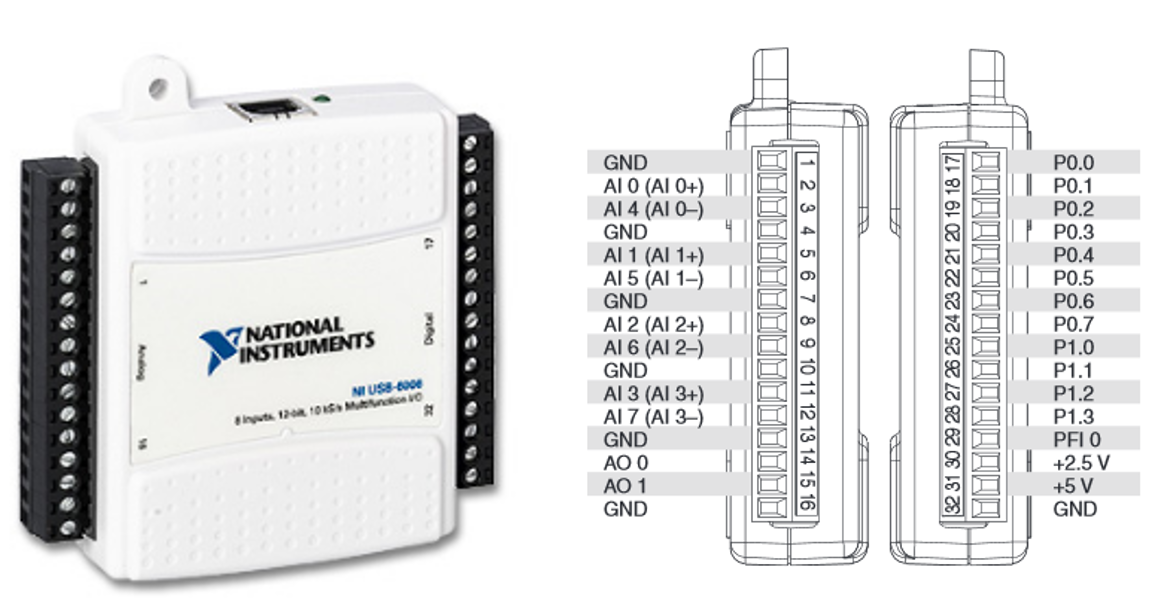
\includegraphics[width=1\linewidth]{Lab8_NationalInstrumentsUSB6009}
\caption{National Instruments NI6009 data acquisition module. Full specs can be found \href{http://abe-research.illinois.edu/Faculty/grift/ABE425_2015/Specs/USB6008.pdf}{here}.}
\label{fig:Lab8_NationalInstrumentsUSB6009}
\end{figure}

\item Soft calibrate the sensor in an ice bath. Put the sensor in the ice bath \textbf{(make sure you use the insulated sensor, you cannot immerse the naked sensor in water without shorting it out}). Make sure the water has had time to attain the melting ice temperature. Adjust the calibration button in the Front Panel to adjust the temperature to 0 deg C.
\item Construct VI data acquisition model in LabVIEW® using Figures \ref{fig:Lab8_TemperatureMeasurementUsingLabVIEW_FrontPanel} (Front panel) and \ref{fig:Lab8_TemperatureMeasurementUsingLabVIEW_BlockDiagram} (block diagram).
A helpful Introduction on how to build VIs by National Instrument employee Fu Ouyang can be found \href{http://abe-research.illinois.edu/Faculty/grift/ABE425_2016/Labs/Lab8_TemperatureMeasurementUsingLabView/Lab8_TemperatureMeasurementUsingLabView_InstructionOfBuildingVI_draft.pdf}{here}.\\ 

a.	Take one voltage reading from the sensor every second.\\
b.	Convert the voltage reading to Kelvin, degrees Celsius, Fahrenheit, and display them.\\
c.	Keep track of and display (in seconds) the elapsed time since the VI was started.\\
d.	Use a waveform chart on the front panel to indicate how the temperature varies with time.\\
e.	Write all of the collected data points to a file when the power switch is turned off.\\
f.	Save your VI in this folder under the name TempTestXX.vi. Let LabVIEW® make a new file for you every time you start the program. Use only one header in the output file.\\

\item Perform the Data Acquisition: With the VI running, allow it to record several seconds of temperature readings when the sensor is at equilibrium with the room.  Then hold the temperature sensor with your fingers and continue to take data until the sensor reaches a new equilibrium temperature.  Release your fingers and wait until the sensor reaches another equilibrium temperature. 
\item Present the Test Results: Save the data to a file and plot the results using Excel.  

\end{enumerate}

\begin{figure}
\centering
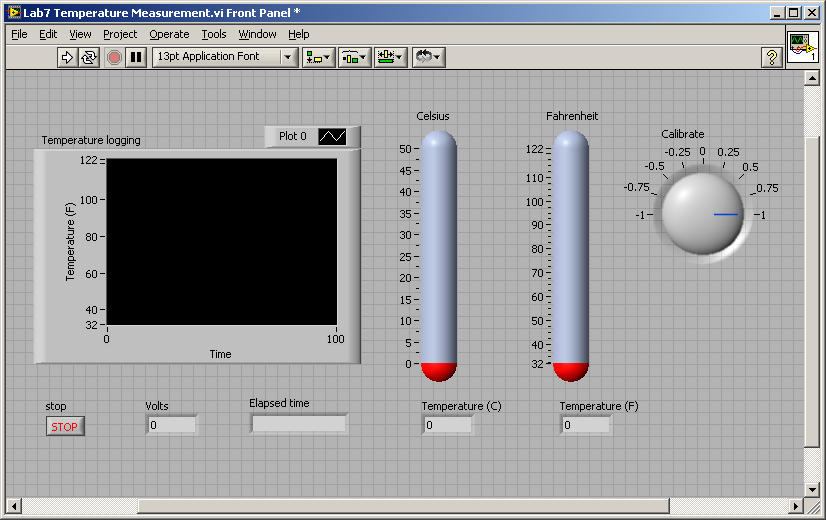
\includegraphics[width=1\linewidth]{Lab8_TemperatureMeasurementUsingLabVIEW_FrontPanel}
\caption{Front panel of the temperature measurement program.}
\label{fig:Lab8_TemperatureMeasurementUsingLabVIEW_FrontPanel}
\end{figure}

\begin{figure}
\centering
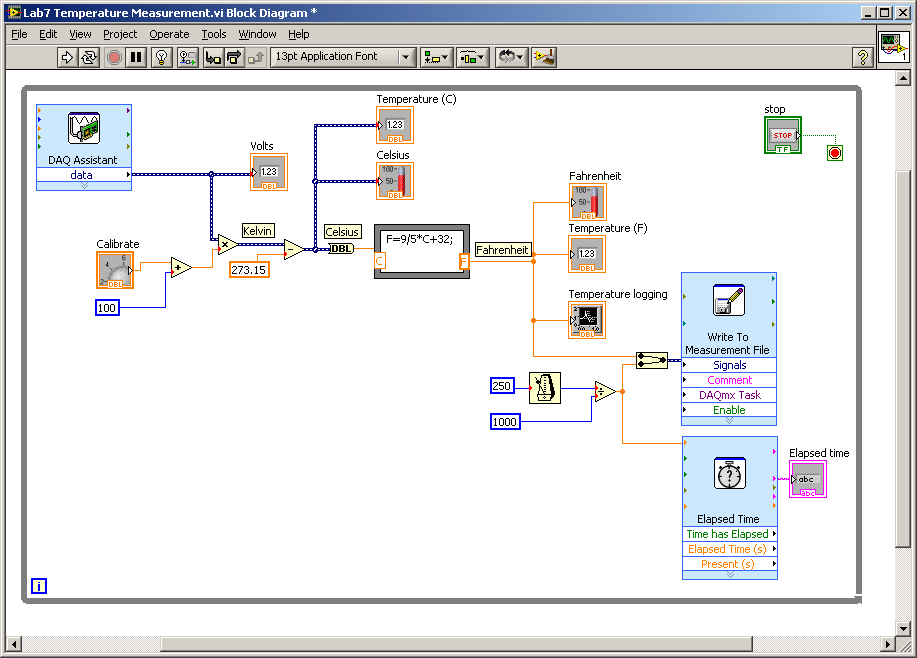
\includegraphics[width=1\linewidth]{Lab8_TemperatureMeasurementUsingLabVIEW_BlockDiagram}
\caption{Block diagram of the temperature measurement program.}
\label{fig:Lab8_TemperatureMeasurementUsingLabVIEW_BlockDiagram}
\end{figure}
 
\section{Questions}

Q1: The International Temperature Scale of 1990 defines several triple points that can be used for temperature calibration. Find the two closest to the triple point of water (0.01 deg C).\\
A1:\\

Q2:	If the voltage drop across the 135 chip is 2.7 Volt, what is a reasonable value of the resistor to limit the current to 0.4 mA?\\
A2:\\


Q3:	What is the current SI definition of temperature? How will it be defined in the future?\\ 
A3:\\

\end{document}
